\setcounter{section}{14}


\section{Lecture 15: Feb 22}


\subsection*{Last time}
\begin{itemize}
  \item Probability review
  \item Lab session
\end{itemize}


\subsection*{Today}
\begin{itemize}
 \item Dummy-Variable regression
 \item Interactions
% \item 2nd-round linear algebra review
\end{itemize}

\subsection*{Dummy-variable regression}
For categorical data (factor), we use dummy variable regression:
$$
Y_i = \beta_0 + \beta_1 X_{i} + \beta_2 D_{i} + \epsilon_i
$$
where $D$, called a \underline{dummy variable} regressor or an \underline{indicator variable}, is coded $1$ for one level and $0$ for all others,
$$
D_i = \left\{ \begin{array}{l l} 1 & \mbox{for men}\\ 0 & \mbox{for women}\\ \end{array} \right. .
$$
Therefore, for women, the model becomes
$$
Y_i =\beta_0 + \beta_1 X_{i} + \epsilon_i
$$
and for men
$$
Y_i = \beta_0  + \beta_1 X_{i} + \beta_2 + \epsilon_i = (\beta_0 + \beta_2) + \beta_1 X_{i} + \epsilon_i
$$

For example, Figure~\ref{fig:income_education_gender} (a) and (b) represents two small (idealized) populations.
In both cases, the within-gender regressions of income on education are parallel.
Parallel regressions imply additive effects of education and gender on income: Holding education constant, the ``effect'' of gender is the vertical distance between the two regression lines, which, for parallel lines, is everywhere the same.
%
\begin{figure}[H]
\begin{center}
  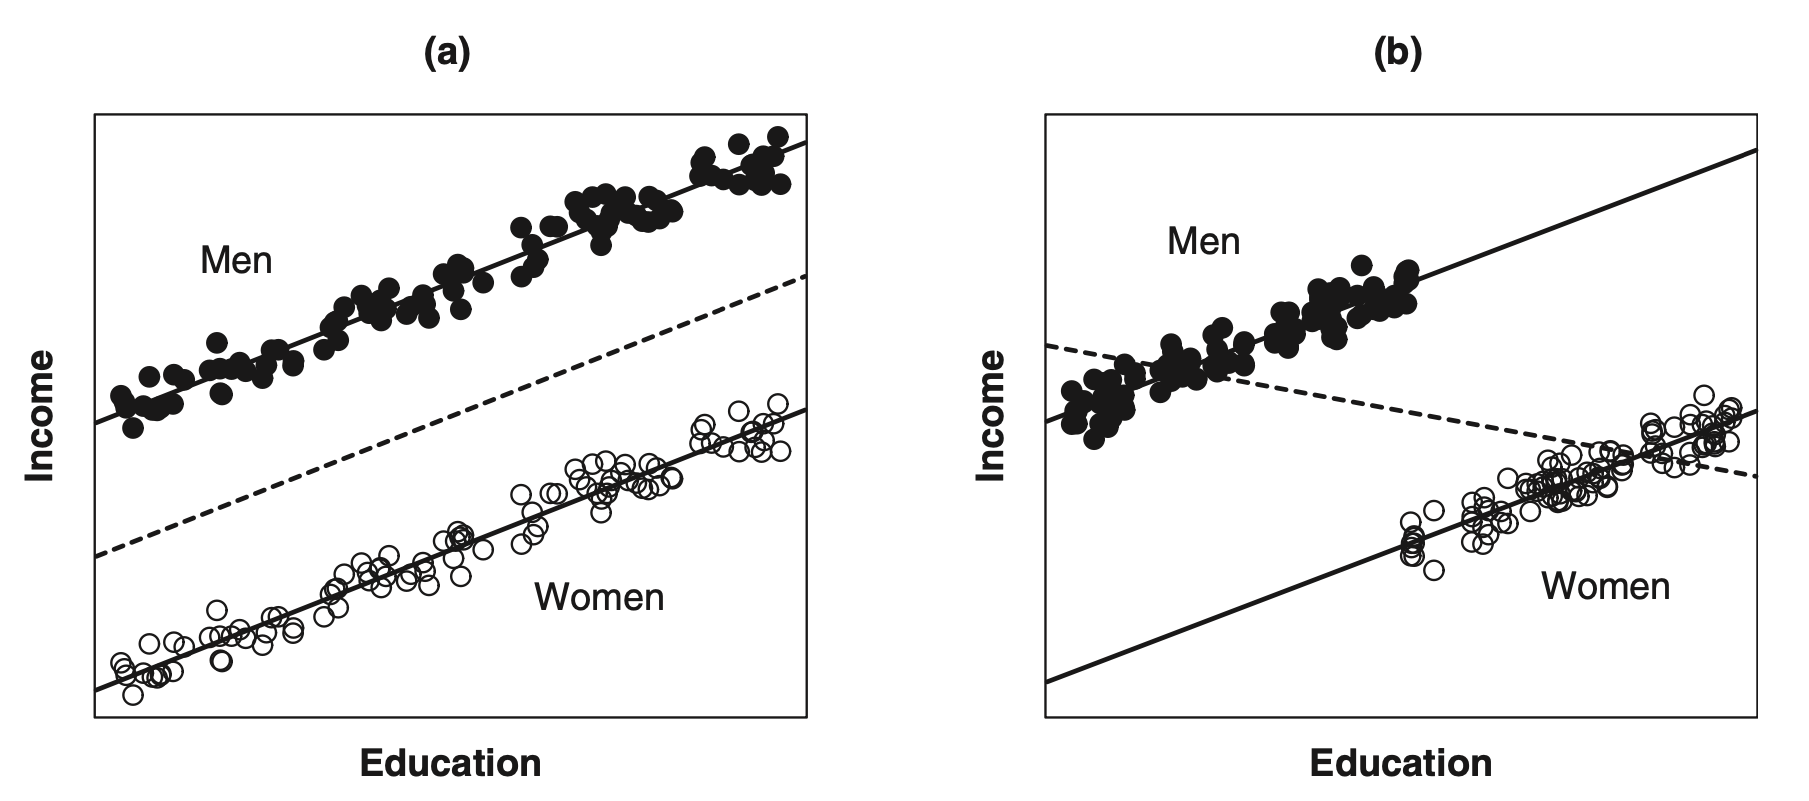
\includegraphics[width=0.8\textwidth]{Lecture15/Figure7_1}
  \caption{Idealized data representing the relationship between income and education for populations of men (filled circles) and women (open circles).  In (a), there is no relationship between education and gender; in (b), women have a higher average level of education than men.
  In both (a) and (b), the within-gender (i.e.,~partial) regressions (solid lines) are parallel.  In each graph, the overall (i.e.~marginal) regression of income on education (ignoring gender) is given by the broken line.
   JF Figure 7.1.}
  \label{fig:income_education_gender}
\end{center}
\end{figure}
%

\subsubsection*{Multi-level factor}

We can model the effects of classification factors with $m$ categories (levels) by using $m-1$ indicator variables.

For example, the three-category occupational-type factor can be represented in the regression equation by introducing two dummy regressors:
\begin{center}
\begin{tabular}{ l c c}
\hline
Category & $D_1$ & $D_2$ \\ 
\hline
Professional and managerial & 1 & 0 \\
White collar & 0 & 1 \\
Blue collar & 0 & 0 \\
\hline
\end{tabular}
\end{center}
%
A model for the regression of prestige on income, education, and type of occupation is then
$$
Y_i = \beta_0 + \beta_1 X_{i1} + \beta_2 X_{i2} + \gamma_1 D_{i1} + \gamma_2 D_{i2} + \epsilon_i
$$
%
where $X_1$ is income and $X_2$ is education.
This model describes three parallel regression planes, which can differ in their intercepts:
$$
\begin{array}{ll}
\mbox{Professional: } & Y_i = (\beta_0 + \gamma_1) + \beta_1 X_{i1} + \beta_2 X_{i2} + \epsilon_i\\
\mbox{White collar: } & Y_i = (\beta_0 + \gamma_2) + \beta_1 X_{i1} + \beta_2 X_{i2} + \epsilon_i \\
\mbox{Blue collar: } & Y_i = \beta_0 + \beta_1 X_{i1} + \beta_2 X_{i2} + \epsilon_i\\
\end{array}
$$
%
Therefore, the coeficient $\beta_0$ gives the intercept for blue-collar occupations; $\gamma_1$ represents the constant vertical difference between the parallel regression planes for professional and blue-collar occupations (fixing the values of education and income); and $\gamma_2$ represents the constant vertical distance between the regression planes for white-collar and blue-collar occupations (again, fixing education and income).

In the above prestige example, we chose ``blue collar'' as the baseline category.
Sometimes, it is natural to pick a particular category as the baseline category, for example, the ``control group'' in an experiment.
However, in most applications, the choice of a baseline category is entirely arbitrary.

\subsubsection*{Matrix representation}
For the above prestige model
$$
Y_i = \beta_0 + \beta_1 X_{i1} + \beta_2 X_{i2} + \gamma_1 D_{i1} + \gamma_2 D_{i2} + \epsilon_i
$$
we have the design matrix $\vecc{X}$ as
$$
\vecc{X} = \left[ \begin{array}{c c c c c} 
1 & X_{11} & X_{12} & D_{11} & D_{12} \\
1 & X_{21} & X_{22} & D_{21} & D_{22} \\
\vdots &\vdots & \vdots & \vdots & \vdots\\
1 & X_{n1} & X_{n2} & D_{n1} & D_{n2} \\
 \end{array}  \right]
$$
and the vector of coefficients $\vecc{\beta}$ is
$$
\vecc{\beta} = \left[ \begin{array}{c} \beta_0\\ \beta_1 \\ \beta_2 \\ \gamma_1 \\ \gamma_2 \\ \end{array} \right]
$$
such that we have (again) the linear model in matrix form:
$$
\vecc{Y} = \vecc{X\beta} + \vecc{\epsilon}
$$
where $\epsilon_i \distas{iid} N(0, \sigma^2)$, in other words,  $\vecc{\epsilon} \sim N(\vecc{0}, \sigma^2 \vecc{I}_n)$.

\subsection*{Interactions}
Two explanatory variables are said to \underline{interact} in determining a response variable when the partial effect of one depends on the value of the other.
Consider the hypothetical data shown in Figure~\ref{fig:interaction}.
%
\begin{figure}[H]
\begin{center}
  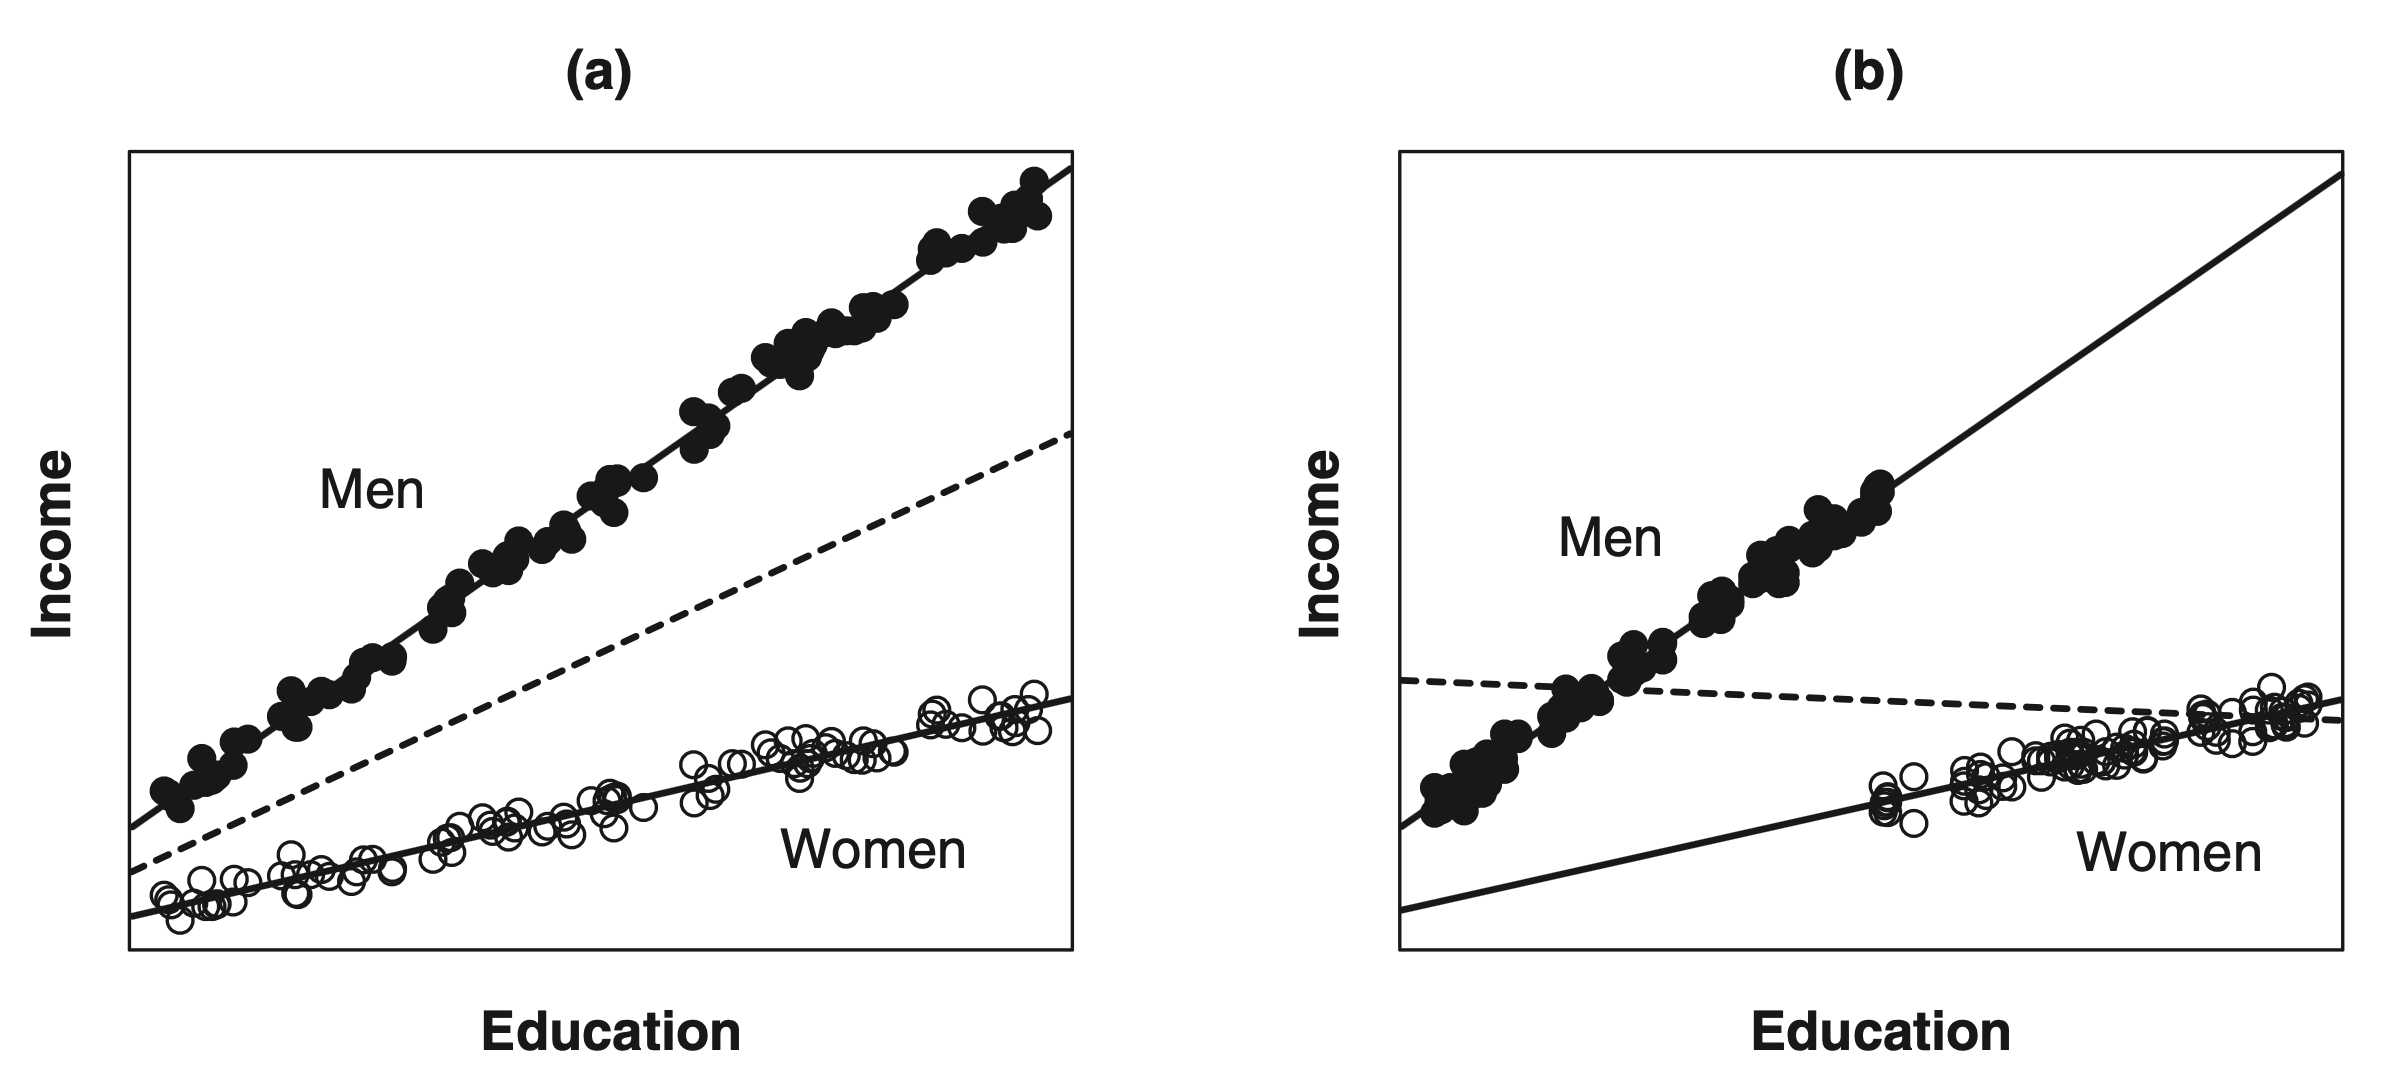
\includegraphics[width=0.8\textwidth]{Lecture15/Figure7_7}
  \caption{Idealized data representing the relationship between income and education for populations of men (filled circles) and women (open circles).
  In (a), there is no relationship between education and gender; in (b), women have a higher average level of education than men.
  In both (a) and (b), the within-gender (i.e.,~partial) regressions (solid lines) are not parallel.
  The slope for men is greater than the slope for women, and consequently education and gender interact in affecting income. 
    In each graph, the overall regression of income on education (ignoring gender) is given by the broken line.
   JF Figure 7.7.}
  \label{fig:interaction}
\end{center}
\end{figure}
%
It is apparent in both Figure~\ref{fig:interaction} (a) and (b) the within-gender regressions of income on education are not parallel: In both cases, the slope for men is larger than the slope for women.

\subsubsection*{Modeling interactions}
We accommodate the interaction of education and gender by:
$$
Y_i = \beta_0 + \beta_1 X_{i} + \beta_2 D_{i} + \beta_3 (X_i D_i) + \epsilon_i
$$
where we introduce the \underline{interaction regressor} $XD$ into the regression equation.
For women, the model becomes
$$
\begin{aligned}
Y_i &= \beta_0 + \beta_1 X_{i} + \beta_2 \cdot 0 + \beta_3 (X_i \cdot 0) + \epsilon_i\\
&= \beta_0 + \beta_1 X_i + \epsilon_i\\
\end{aligned}
$$
%
and for men
$$
\begin{aligned}
Y_i &= \beta_0 + \beta_1 X_{i} + \beta_2 \cdot 1 + \beta_3 (X_i \cdot 1) + \epsilon_i\\
&= (\beta_0 + \beta_2) + (\beta_1 + \beta_3) X_i + \epsilon_i\\
\end{aligned}
$$
The parameters $\beta_0$ and $\beta_1$ are, respectively, the intercept and slope for the regression of income on education among women (the baseline category for gender);
$\beta_2$ gives the difference in intercepts between the male and female groups;
and $\beta_3$ gives the difference in slopes between the two groups.

{\it Usual guidance: } Models that include an interaction between two predictors should also include the individual predictors by themselves regardless of the statistical significance of the associated $\beta$'s.

\subsubsection*{Test for the interaction}
We can simply test the hypothesis $H_0: \beta_3 = 0$ and construct the test statistic $t = \frac{\hat{\beta}_i - 0}{\reallywidehat{SE}(\hat{\beta}_i) } \sim t_{n - 4}$ ($p = 3$).

\subsubsection*{Interactions with multi-level factor}
We can easily extend the method for modeling interactions by forming product regressors to multi-level factors, to several factors, and to several quantitative explanatory variables.
Using the occupational prestige example, the occupational type could possibly interact both with income ($X_1$) and with education ($X_2$):
$$
\begin{aligned}
Y_i = \beta_0 &+ \beta_1 X_{i1} + \beta_2 X_{i2} + \gamma_1 D_{i1} + \gamma_2 D_{i2} \\
 &+\delta_{11} X_{i1} D_{i1} +\delta_{12} X_{i1} D_{i2} +\delta_{21} X_{i2} D_{i1} +\delta_{22} X_{i2} D_{i2} + \epsilon_i\\
\end{aligned}
$$
The model therefore permits different intercepts and slopes for the three types of occupations:
$$
\begin{array}{lrrrrr}
\mbox{Professional: } & Y_i = &(\beta_0 + \gamma_1) + &(\beta_1 + \delta_{11}) X_{i1} +& (\beta_2 + \delta_{21}) X_{i2}  +&\epsilon_i\\
\mbox{White collar: } & Y_i = &(\beta_0 + \gamma_2) + &(\beta_1 + \delta_{12}) X_{i1} +& (\beta_2 + \delta_{22}) X_{i2}  +&\epsilon_i\\
\mbox{Blue collar: } & Y_i = &\beta_0 + &\beta_1 X_{i1}+ & \beta_2 X_{i2}  +&\epsilon_i\\
\end{array}
$$











